\section{Dosímetro Active Pixel Sensor}
\fig{aps}{esquematicos/aps.pdf}{Esquemático del dosímetro APS}
El dosímetro APS tiene una estructura similar a 
un pixel del sensor de imagen en una cámara digital. 
Requiere alimentación durante la irradiación,
pero puede operar con tensiones pequeñas
como las que provee una batería.
Asimismo, tiene la ventaja de poder resetearse rápidamente.
Esto permite tomar mediciones con gran resolución temporal.

Esta parte del trabajo comienza con la teoría del dosímetro.
Luego cubre cómo realizamos el diseño y lo optimizamos.
Por último, presenta las mediciones del sensor fabricado 
y las conclusiones que siguen de ellas.
%
\subsection{Principio de funcionamiento}
%
Su principio de funcionamiento es medir 
la carga generada por radiación 
en la zona desierta de una juntura p-n.
El cátodo de la juntura está aislado eléctricamente 
para acumular la carga generada sin que se fugue
(D1 en \figref{fig:aps}).
Antes de cada medición, se reinicia el circuito llevando dicho cátodo a
V$_{\text{DD}}$ prendiendo brevemente el transistor de reset M1.
La radiación que incide en la zona desierta de D1 interactúa con la red de
silicio, depositando energía a través de distintos procesos como scattering e
ionización (ver sección~\ref{sec:radiacion}).
Los fotones y electrones secundarios resultantes producen pares electrón-hueco,
que son arrastrados en direcciones opuestas por el campo eléctrico
que existe normalmente en la zona desierta.
Los electrones se acumulan en el cátodo,
descargándolo gradualmente hacia \SI{0}{\volt}.
Luego de irradiar,
se mide su tensión a través de un par de seguidores M2 y M3.
Los mismos forman un circuito que replica la tensión de entrada a la salida,
pero desplazada un valor fijo.
Su propósito es evitar que la medición de tensión modifique la carga en el nodo y
afecte al valor medido.
\subsection{Trabajos previos}
Turchetta\cite{turchetta_monolithic_2001} describe un APS para rayos X
construído en un proceso CMOS estándar de \SI{0.6}{\micro\meter}. 
Construye una grilla de píxeles para uso en tracking de partículas.
Expone el sensor a rayos X provenientes de \isotope{Fe}{55},
y a piones de \SI{15}{\giga\electronvolt}.
Expresa la sensibilidad en términos de Volts por electrón generado por
radiación. Esta figura llega a \SI{15}{\micro\volt} por electrón,
con un ruido RMS equivalente a 15 electrones.
Una innovación es el uso de un layout que permite que casi toda la superficie
del wafer sea sensible.

Matis\cite{matis_charged_2003} también construye un array de APS,
en un proceso estándar de \SI{0.25}{\micro\meter}.
Analiza distintas formas de procesar la señal,
sumando la salida de varios píxeles para colectar toda la carga generada por
una partícula incidente.
Irradia el sensor con rayos X provenientes de \isotope{Fe}{55},
y protones de \SI{55}{\mega\electronvolt}.

Conti\cite{conti_use_2013} emplea un sensor de imagen CMOS comercial
para estudiar su respuesta a rayos X.
En particular, analiza la distribución 2D generada por un fotón
y otras estadísticas.
Usa como fuente de radiación un equipo de radioterapia,
y simula el scattering producido por el paciente usando un bloque de acrílico
como phantom.
%
\subsection{Proceso de fabricación}
Si bien la fabricación viene luego del diseño,
todo el diseño está condicionado por 
las características del proceso de fabricación.
En específico,
\begin{itemize}
    \item qué tensiones soporta,
    \item qué dispositivos provee, y
    \item qué características eléctricas tienen esos dispositivos
        (tensiones umbral, capacidades parásitas, corrientes de pérdida, etc).
\end{itemize}

Diseñamos y mandamos a fabricar tanto el FG como el APS 
en el proceso XC06 de la foundry X-FAB \cite{x-fab_0.6_2008}.
El mismo tiene una tecnología (longitud característica) 
de \SI{0.6}{\micro\meter} 
y está diseñado para tensiones de hasta \SI{5}{\volt}.
En su versión estándar, 
cuenta con 1 capa de polisilicio y 2 de metalización.
Existen variantes del proceso que utilizan máscaras adicionales para,
por ejemplo, abrir ventanas para formar regiones fotosensibles.
\subsection{Reset}
Se carga el nodo flotante a través del drain de un MOSFET de canal P,
con el source conectado a \vdd (\figref{fig:aps}).
Durante la irradiación se lleva su gate a \vdd, apagándolo.
Para resetear 
se lleva su gate a tierra.
Esto lo coloca en saturación,
cargando la juntura a corriente constante 
y aumentando $V_D$ linealmente hasta $V_t$.
Entonces entra en triodo y va reduciendo la corriente,
cargando asintóticamente hasta \vdd.
Esto permite llevarlo a $V_{dd}$,
mientras que una llave de tipo N sólo llegaría hasta $V_{dd}-V_{tn}$ antes de
apagarse.

El transistor de reset es de área mínima,
para que aporte la menor capacidad parásita posible al nodo flotante.
Esto, como se verá más adelante, maximiza la sensibilidad del sensor.
\subsection{Respuesta a partículas}
Cada partícula incidente deposita una energía promedio que depende de su energía
cinética inicial\cite{berger_response_1969} (ver sección~\ref{montecarloaps}).
Una fracción $E$ de esta energía se usa en la creación de pares electrón-hueco,
generando carga 
\begin{align*}
    Q &= \frac{qE}{E_i}
\end{align*}
con $q$ la carga del electrón y $E_i$ la energía de creación de pares,
\SI{3.62}{\electronvolt} en Si.
Esta carga aparece con signo negativo en el cátodo, descargándolo.
Su cambio de tensión
\begin{align*}
    \Delta V &= \frac{\Delta Q}{C}
\end{align*}
depende de la capacidad total $C$ del nodo.
La misma tiene contribuciones de
\begin{itemize}
    \item juntura de D1,
    \item juntura Drain-Body de M1,
    \item Gate de M2, y
    \item conductores cercanos al nodo.
\end{itemize}
Estas capacidades pueden estimarse a partir de las especificaciones del 
proceso de fabricación,
que indican capacidad por unidad de área y por unidad de perímetro.
Para eso usamos herramientas de EDA (electronic design automation)
que realizan esta estimación automáticamente a partir de la geometría del
diseño (ver sección~\ref{section:diseno_aps}).
\subsection{Cálculos Monte-Carlo}
\label{montecarloaps}
El dosímetro APS detecta energía depositada 
en una región específica de un circuito integrado.
A fines de simularlo, 
simplificamos la geometría del die en tres regiones:
una superficie de SiO$_2$, un sustrato de Si 
y una zona sensible también de Si (\figref{fig:corteaps}).
\fig{corteaps}{figuras/aps/corte.pdf}
{Corte de la geometría usada para simular el APS en Geant4 (no a escala).}
Las dimensiones se extrajeron del diseño del APS 
y de las especificaciones del proceso de fabricación del chip.

Dado que el uso principal de Geant4 es en física de altas energías,
su configuración por defecto no permite simular electrones secundarios por
debajo de \SI{250}{\electronvolt}.
% DETAIL rango a 250eV ~ nm, qué me importa?
Para obtener precisión a escalas de distancia más chicas,
empleamos una lista de procesos de interacción 
compilada para simulaciones en microelectrónica \cite{Raine201497}.
La misma simula con fidelidad electrones hasta \SI{16.7}{\electronvolt},
cuyo rango en Si es del orden de \SI{0.1}{\nano\meter}.

Los resultados se encuentran en la \figref{fig:energia1electron}.
% FIXME falta este gráfico usando
% ../tesis/figuras/aps/deposicion1electron001.pdf y demás
\fig{energia1electron}{figuras/aps/deposicion1electron_todos.pdf}
{Distribución de probabilidad simulada en Geant4 
    para la energía depositada en el sensor (eje X).
Cada gráfico corresponde a una dada energía cinética de la partícula incidente.
La energía promedio depositada está en la \figref{fig:energiadepositadaaps}.}
El aumento de la respuesta al reducir la energía incidente se debe a que 
los electrones menos energéticos 
tienden a frenarse por completo en el detector,
depositando toda su energía.
Los más energéticos, en cambio, depositan una fracción variable de su energía
total.
La energía depositada promedio se encuentra en la
\figref{fig:energiadepositadaaps}.
\fig{energiadepositadaaps}{figuras/poster/aps_respuesta.pdf}
{Respuesta promedio a un electrón incidente,
en función de su energía inicial.
Se ve que los electrones menos energéticos se frenan completamente en el
detector.
Las cruces son el resultado de simulación con Geant4,
mientras que la línea es un cálculo manual 
con los datos tabulados por NIST en ESTAR\cite{berger_estar_????}.}
Se ve que para el rango de energías de interés,
cada partícula incidente produce un cambio de decenas de mV.
\subsection{Fuentes de ruido}
El APS se maneja con corrientes y variaciones de carga y tensión muy
pequeñas.
Por eso es crítico conocer los procesos que introducen ruido, 
y su magnitud.
Este ruido se combina con la señal proveniente de la radiación
y determina la resolución del dosímetro: 
la dosis mínima que es posible resolver por encima del
ruido\cite{taylor_introduction_1997}.
\subsubsection{Corriente de fuga de juntura p-n}
Al polarizar una juntura p-n en inversa, fluye una corriente de
pérdida\cite{sze_physics_2007} con un valor de DC dado por
\begin{align*}
    I&=I_s(e^{\frac{qV}{\eta kT}}-1)
\end{align*}
con $V<0$ la tensión aplicada y $I_s$ y $\eta$ parámetros de fabricación de la
juntura.
El valor instantáneo de $I$ fluctúa debido a la naturaleza discreta de los portadores que
atraviesan la barrera de energía de la juntura.
Esta fluctuación se denomina ruido \emph{shot}, una clase de ruido blanco:
su densidad espectral de potencia,
\begin{align*}
    i^2(f) &= 2q|I|,
\end{align*}
no varía con la frecuencia (hasta frecuencias muy altas).
\subsubsection{Fluctuaciones durante reset}
Durante el reset, se carga la juntura p-n hasta $V_{dd}$ a través de M1.
Cerca de la tensión final, M1 entra en modo triodo.
En esta condición de operación, el canal actúa como una resistencia.
Esto significa que produce ruido de Johnson\cite{baker_cmos_2010}.
Al cargar la capacidad de juntura $C$, 
este ruido produce una varianza en la tensión final dada por
\begin{align*}
    \overline{v^2} &= \frac{kT}C.
\end{align*}
Evaluando esta fórmula con la capacitancia del APS
% TODO: es la capacidad de 4x4 o 40x40?
se llega a una tensión de ruido RMS de \SI{1.1}{\milli\volt}.

Esta incertidumbre en la tensión luego del reset puede eliminarse usando 
la técnica Correlated Double Sampling\cite{white_characterization_1974}:
se mide tensión antes y después de la exposición a la radiación.
Al tomar la diferencia se elimina el ruido de reset,
presente en ambas por igual.

\subsection{Diseño del circuito}
\label{section:diseno_aps}
La topología del circuito quedó determinada por la elección de construir un
dosímetro APS con un par de seguidores para su medición.
El paso siguiente en el diseño fue elegir los tamaños de los distintos
componentes para optimizar el desempeño del sensor.

Para una carga dada, la tensión sobre un capacitor es inversamente proporcional
a su capacidad.
En el APS la carga es generada por la radiación,
y la tensión es la señal cuya magnitud queremos maximizar.
Para esto minimizamos las capacidades parásitas del cátodo de D1,
usando transistores de área mínima para M1 y M2.
Restringimos el largo de las conexiones del cátodo,
y las mantuvimos alejadas de otros nodos.
Aplicamos software de Mentor de extracción de capacidades parásitas al layout
resultante, y obtuvimos una capacidad total en el cátodo de \SI{3.4}{\femto\farad}.

El tamaño del primer MOS seguidor, M2, 
tiene que ser el tamaño mínimo para no cargar capacitivamente
al nodo que acumula carga.
Esto deja libre las dimensiones del segundo MOS seguidor, M3.
Mientras más grande es, mayor es su capacidad de gate
y por lo tanto más va a cargar a la etapa anterior.
Por otro lado va a tener mayor capacidad de corriente
para manejar la carga capacitiva del pad de salida.

Estimamos un tamaño inicial para M3 fijando un largo arbitrario
y variando el ancho para minimizar una figura de mérito.
La figura que elegimos representa el delay producido por los dos seguidores,
\begin{align}
    \tau &= \tau_1+\tau_2 = g_{m2}C_{g3} + g_{m3}C_{\textnormal{pad}}
    \label{eq:delay_seguidor_aps}
\end{align}
con $g_m=\pderiv{I_D}{V_G}$ la transconductancia de un MOS 
y $C_g$ su capacidad de gate.
Minimizando la ecuación~\ref{eq:delay_seguidor_aps}
para una polarización pre-fijada,
llegamos a un $W$ inicial de \SI{409}{\micro\meter}.

El paso siguiente es hacer un cálculo más preciso 
que incluya todos los detalles del funcionamiento del circuito.
Para esto simulamos con SPICE el tiempo de respuesta a un electrón incidente
en función del ancho de M3 (\figref{fig:falltime}).
\fig{falltime}{figuras/aps/falltime.pdf}
{Tiempo de respuesta simulado del buffer en función del ancho del MOS del
    segundo seguidor. 
    $W_{\textnormal{ideal}}$ es el $W$ óptimo cálculado a mano de forma
    simplificada.
}
Se ve que hay poca mejora en el tiempo de respuesta 
al aumentar $W$ por encima de nuestro estimado inicial.
Por eso, teniendo en cuenta las limitaciones de área,
elegimos un ancho total de \SI{400}{\micro\meter} repartido entre 8 canales 
(o sea 8 MOS en paralelo, cada uno de \SI{50}{\micro\meter}).

Las dimensiones finales están en la tabla~\ref{fig:areas_aps}.
Incluímos también una variante con un diodo más grande,
de modo que su capacidad opaque las otras capacidades parásitas.
\begin{table}[h]
    \centering
    \caption{Dimensiones del diseño optimizadas para sensibilidad y tiempo de
    respuesta}
    \begin{tabular}{|c|c|c|c|}
        \hline
        Dispositivo&      W (um)&    L (um)&  Canales\\
        \hline
D1&     4&  4&  1\\
M1&     0.8&    0.6&    1\\
M2&     0.8&    0.6&    1\\
M3&     50& 3&  8\\
        \hline
    \end{tabular}
    \label{fig:areas_aps}
\end{table}

Estas dimensiones se utilizaron tanto para la simulación del circuito en SPICE
como para los cálculos Monte-Carlo.
La combinación de estas dos herramientas nos da una sensibilidad esperada de 
\SI{7.1}{\volt\per\gray}.
El diseño físico final está en la \figref{fig:layoutaps},
y el esquemático en la \figref{fig:aps}.
\begin{figure}[p]
    \centering
    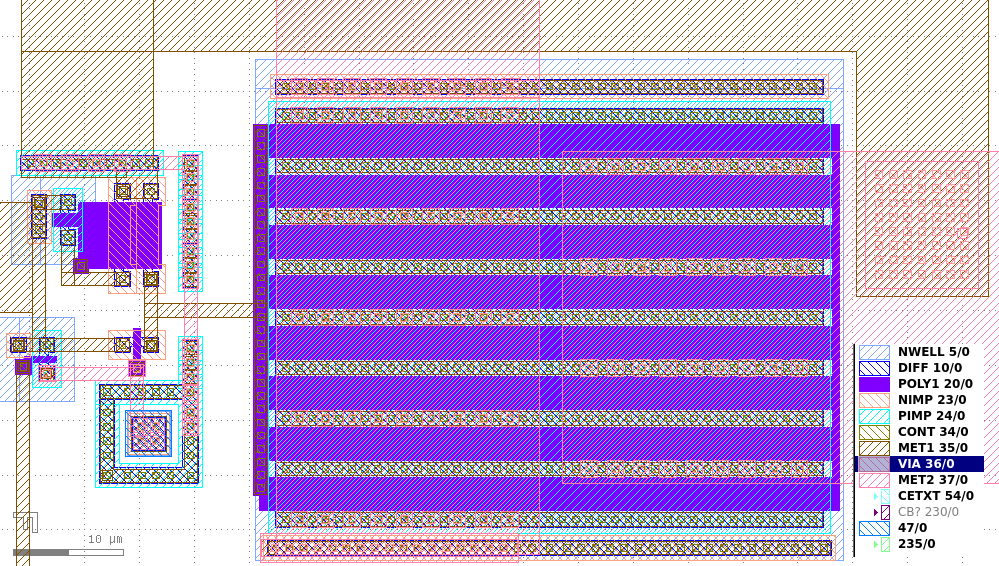
\includegraphics[width=\columnwidth]{figuras/gds/aps/todo.png}
    \caption{Layout del dosímetro APS. 
    El transistor de la derecha es el de salida, del segundo seguidor.
    El resto se ve en más detalle en la \figref{fig:layoutapszoom}.}
    \label{fig:layoutaps}
\end{figure}
\begin{figure}[p]
    \centering
    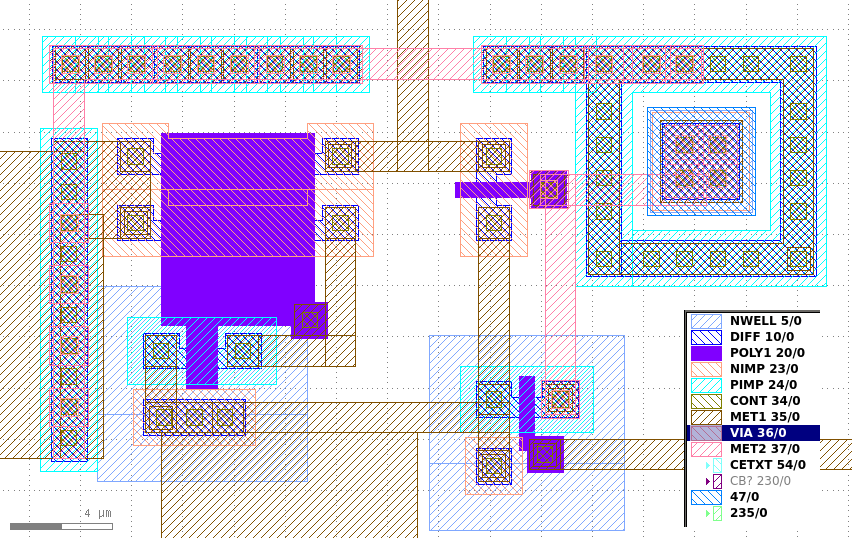
\includegraphics[width=\columnwidth]{figuras/gds/aps/zoom.png}
    \caption{Vista en detalle del layout del APS, excluyendo el transistor de
        salida.
        A la derecha está el diodo, con el cátodo (nwell) en el centro y el
        ánodo (contactos a sustrato) rodeándolo.
        A su izquierda está el primer MOSFET seguidor y abajo el MOSFET de
        reset.
        Los transistores de la izquierda polarizan al primer seguidor.
    El transistor de reset está conectado a un pad (no visible) a través del
    circuito de protección de la \figref{fig:proteccion5v}.}
    \label{fig:layoutapszoom}
\end{figure}
\fig{proteccion5v}{figuras/aps/proteccion.pdf}
{Circuito de protección para la entrada de reset.
Los diodos sólo conducen si la tensión del pad excede \SI{5}{\volt} o
baja de \SI{0}{\volt}.
Cuando llega un pulso de alta tensión
(por ejemplo debido a una descarga electrostática)
los diodos limitan la tensión que llega al circuito.
Esto evita que se polaricen en directa las junturas drain-body y source-body,
previniendo una falla por latchup (sección~\ref{latchup}).
También evita la ruptura de los óxidos de compuerta de MOS.}
\subsection{Medición}
Tomamos dos dies y los bondeamos a placas adaptadoras de TSSOP28,
un tipo de empaquetado de circuitos integrados de montaje superficial
(figuras~\ref{fig:bondeados1}, \ref{fig:bondeados2} y~\ref{fig:pinout}).
\fig{bondeados1}{figuras/aps/bondeados.jpg}
{Dies bondeados a placa adaptadora SMD.
Los zócalos tienen las patas cortocircuitadas para proteger al die de
descargas electrostáticas durante el transporte y almacenamiento.}
\figp{bondeados2}{figuras/aps/die.jpg}
{Detalle del die fabricado con los dosímetros APS y FG 
(arriba en la columna central)
y otros circuitos.}
\figp{pinout}{figuras/aps/pinout1.pdf}
{Layout del die entero con numeración de los pads bondeados}
\subsubsection{Descarga en oscuridad}
Primero medimos la respuesta del sensor sin luz ni radiación
(figuras~\ref{fig:oscuridad4} y~\ref{fig:oscuridad40}).
\fig{oscuridad4}{figuras/aps/oscuridad4.pdf}
{Curva de descarga en oscuridad del APS de 4x\SI{4}{\micro\meter}.
Resulta de resetear el APS y medir su tensión de salida en oscuridad.}
\fig{oscuridad40}{figuras/aps/oscuridad40.pdf}
{Curva de descarga en oscuridad del APS de 40x\SI{40}{\micro\meter}.
Resulta de resetear el APS y medir su tensión de salida en oscuridad.}
Esto nos muestra la descarga del diodo debido a la corriente de fuga en
inversa.

Se ve en ambas figuras la misma curva 
con escalas distintas de tiempo y de tensión.
Esta variación proviene tanto de las áreas distintas de los dos sensores
como de las variaciones aleatorias entre los MOS seguidores (mismatch).
Cada transistor del die tiene pequeñas variaciones debido a imperfecciones en
la litografía y variaciones aleatorias de dopaje.
Estas variaciones no son tan notables en dispositivos grandes debido a que
se cancelan al promediarse sobre mucha área.

Ya que los seguidores usan varios transistores de área mínima,
son particularmente sensibles a variaciones del proceso:
el mismo error absoluto en las dimensiones del canal produce un mayor error relativo.

% Descarga debería ser lineal
% https://books.google.com.ar/books?id=6Rg7AAAAQBAJ&lpg=PA289&ots=yO1HPv_N4E&dq=reverse%20biased%20diode%20%22discharge%20curve%22&hl=es&pg=PA290#v=onepage&q=reverse%20biased%20diode%20%22discharge%20curve%22&f=false

La curva de descarga es la solución a una ecuación diferencial
no-lineal:
\begin{align*}
    \frac{\partial Q}{\partial V}\frac{dV}{dt} &= -I(V)
\end{align*}
La forma de la curva proviene de la variación 
tanto de la corriente de fuga $I(V)$ 
como de la capacidad del diodo $\frac{\partial Q}{\partial V}(V)$.
Ambas dependen de la tensión aplicada,
debido a la variación del ancho de la zona desierta.
Al caer la tensión en inversa,
la zona desierta se vuelve más angosta.
Esto reduce su volúmen y por lo tanto 
la tasa de generación térmica de pares electrón-hueco.
Por otra parte,
su capacidad es inversamente proporcional a este ancho.
Ambos fenómenos reducen la tasa de descarga,
como se ve al final de ambas curvas.

Por otro lado, hay factores de segundo orden 
que no contemplamos en el análisis.
Por ejemplo, el transistor de reset apagado
no es un circuito abierto perfecto, 
sino que tiene una corriente de pérdida muy pequeña.
Esta corriente va a tender a cargar el cátodo de D1,
enlenteciendo la descarga.
%
\subsection{Iluminación con LED}
Medimos las curvas de descarga iluminando los dies con un LED,
variando su corriente para lograr distintas intensidades de iluminación
(figuras~\ref{fig:led4} y~\ref{fig:led40}).
\fig{led4}{figuras/aps/descarga_led_4.pdf}
{Curva de descarga iluminando con un LED el APS de 40x\SI{40}{\micro\meter}.
La corriente del LED aumenta de \SI{.1}{\milli\ampere} a la derecha hasta
\SI{10}{\milli\ampere} a la izquierda,
con 6 curvas por década.}
\fig{led40}{figuras/aps/descarga_led_40.pdf}
{Curva de descarga iluminando con un LED el APS de 4x\SI{4}{\micro\meter}.
La corriente del LED aumenta de \SI{.1}{\milli\ampere} a la derecha hasta
\SI{10}{\milli\ampere} a la izquierda,
con 6 curvas por década.}
Esto permite observar la compresión en tiempo de la curva de descarga 
con el aumento de la radiación incidente.
No fue posible medir el efecto de otros tipos de radiación
(por ejemplo, $\beta$) por limitaciones de tiempo.
\subsubsection{Ruido medido}
Establecimos que una medición con este dosímetro consiste en promediar 10
muestras de tensión.
Esto nos permite definir de manera precisa el ruido como la desviación estándar
de ese promedio.
Más precisamente, la tensión de salida a tasa de dosis constante
es la suma de una componente determinista $V_D$ y una aleatoria $\epsilon$
\begin{align*}
    V = V_D(\dot D, t) + \epsilon
\end{align*}. 
Al tomar la diferencia entre dos muestras consecutivas,
queda una pequeña componente sistemática 
(proporcional a $\Delta t\partial{V_D}{t}$) 
sumada a la diferencia entre dos variables aleatorias que suponemos
independientes.
Por lo tanto, 
la desviación estándar de la diferencia entre dos muestras consecutivas
es $\sqrt 2$ veces la desviación estándar presente en una muestra.

Calculamos esa desviación estándar en base a las curvas medidas
(figuras~\ref{fig:ruido4} y~\ref{fig:ruido40}).
% TODO De dónde sale la equivalencia? ¿Es este sigma representativo de la
% dispersión en una repetición de disparos? Diría que está restringido a la
% freq de muestreo
\fig{ruido4}{figuras/aps/ruido4.pdf}{Ruido a la salida del APS de
    \SI{4x4}{\micro\meter}, calculado tomando diferencias entre muestras
    consecutivas y
escalando para que represente el ruido en un promedio de 10 valores.
La dosis equivalente se calculó con la sensibilidad proveniente
de las simulaciones SPICE y los cálculos de radiación.}
\fig{ruido40}{figuras/aps/ruido40.pdf}{Ruido a la salida del APS de
    \SI{40x40}{\micro\meter}, calculado tomando diferencias entre muestras
    consecutivas y
escalando para que represente el ruido en un promedio de 10 valores.
La dosis equivalente se calculó con la sensibilidad proveniente
de las simulaciones SPICE y los cálculos de radiación.}
Podemos convertir estos valores de ruido en dosis usando la sensibilidad
calculada en~\ref{section:diseno_aps}.
Así llegamos a una resolución de \SI{2.0}{\milli\gray} y \SI{2.3}{\milli\gray}
para el APS de \SI{4x4}{\micro\meter} y \SI{40x40}{\micro\meter},
    respectivamente.

Este análisis del ruido no contempla todas los formas posibles
de usar el APS.
Su validez principal es al realizar una medición Correlated Double Sampling,
restando la tensión final a la tensión luego del reset.
Sin embargo,
también existe la posibilidad de medir durante intervalos largos,
sumando la dosis medida en cada ciclo de reset y descarga.
En este caso, se suma el error en cada disparo para llegar a un valor de ruido
proporcional a la raíz de la cantidad de disparos.
%
\subsection{Resúmen de características}
El dosímetros APS de \SI{4x4}{\micro\meter} que diseñamos, 
fabricamos y construímos presenta las
siguientes características:
\begin{itemize}
    \item Sensibilidad: \SI{7.1}{\volt\per\gray}
    \item Resolución: \SI{2.0}{\milli\gray}
    \item Rango (por disparo): \SI{0.4}{\gray}
\end{itemize}
%
\subsection{Conclusiones}
Presentamos el concepto básico del dosímetro APS,
con sus peculiaridades de uso y el tipo de mediciones que permite realizar.
Cubrimos su teoría de funcionamiento,
y de ahí explicamos el proceso de diseñar el circuito
para su fabricación.

En los resultados verificamos que el sensor
sigue el comportamiento básico que esperamos,
tanto en ausencia de radiación 
como para distintas intensidades de luz visible.
Asimismo, conseguimos una estimación inicial de la resolución del sensor
en base al ruido medido a la salida.
Así dimos los primeros pasos para implementar un dosímetro APS
en un proceso de fabricación CMOS estándar.
